%----------------------------------------------------------------------------------------
%	PACKAGES AND THEMES
%----------------------------------------------------------------------------------------

\documentclass[aspectratio=169]{beamer}

\mode<presentation> {

\usetheme{Madrid}

%\setbeamertemplate{footline} % To remove the footer line in all slides uncomment this line
%% \setbeamertemplate{footline}[page number] % To replace the footer line in all slides with a simple slide count uncomment this line

\setbeamertemplate{navigation symbols}{} % To remove the navigation symbols from the bottom of all slides uncomment this line
}

\usepackage{graphicx} % Allows including images
\usepackage{booktabs} % Allows the use of \toprule, \midrule and \bottomrule in tables

%% Bunch of stuff to make a flowchart with tikz
\usepackage{tikz}
\usetikzlibrary{matrix,calc,shapes,arrows}
\tikzset{
  treenode/.style = {shape=rectangle, rounded corners,
    draw, anchor=center,
    text width=5em, align=center,
    top color=white, bottom color=blue!20,
    inner sep=1ex},
  decision/.style = {treenode, diamond, inner sep=0pt},
  root/.style     = {treenode, font=\Large,
    bottom color=red!30},
  env/.style      = {treenode, font=\ttfamily\normalsize},
  finish/.style   = {root, bottom color=green!40},
  dummy/.style    = {circle,draw}
}
\tikzstyle{format} = [draw, thin, fill=blue!20]
\tikzstyle{medium} = [ellipse, draw, thin, fill=green!20, minimum height=2.5em]


\newcommand{\yes}{edge node [above] {yes}}
\newcommand{\no}{edge  node [left]  {no}}

%----------------------------------------------------------------------------------------
%	TITLE PAGE
%----------------------------------------------------------------------------------------

\title[Summary Presentation]{Geoff Rosenberg Interview} % The short title appears at the bottom of every slide, the full title is only on the title page

\author{Geoff Rosenberg} % Your name
\institute[] % Your institution as it will appear on the bottom of every slide, may be shorthand to save space
{
%% \medskip
\textit{Geoff.Rosenberg@gmail.com} % Your email address
}
\date{June 1, 2018} % Date, can be changed to a custom date

\begin{document}

\begin{frame}
\titlepage % Print the title page as the first slide
\end{frame}

\begin{frame}
\frametitle{Overview} % Table of contents slide, comment this block out to remove it
\tableofcontents % Throughout your presentation, if you choose to use \section{} and \subsection{} commands, these will automatically be printed on this slide as an overview of your presentation
\end{frame}

%----------------------------------------------------------------------------------------
%	PRESENTATION SLIDES
%----------------------------------------------------------------------------------------

%------------------------------------------------
\section{Personal Summary} % Sections can be created in order to organize your presentation into discrete blocks, all sections and subsections are automatically printed in the table of contents as an overview of the talk
%------------------------------------------------

%% ** First 20 minutes of the presentation should be a high level overview of myself -- call it a personal statement.
%% *** This is where I talk about why I want to go into the space industry
%% **** Overarching mission is I want the world to benefit from the work I do.  That's why I went into renewable energy, and that's why I want to go into the space industry
%% **** Might want to mention that our team won the robotics competition
%% *** Questions I want to answer
%% **** Why did I choose my schools and degrees?
%% ***** Although UW as actually the first school that I heard back from, I chose San Diego for undergrad because it made more financial sense.
%% ***** USC because it has a highly rated MS program for dynamics and controls
%% **** Why am I changing jobs?
%% ***** I've always wanted to work in space

%% \subsection{Subsection Example} % A subsection can be created just before a set of slides with a common theme to further break down your presentation into chunks

\begin{frame}
  \frametitle{Overarching Mission}
  This is where I'd talk about \textbf{why} I want to go into the space industry.  In a sentence or two.  In essence, it's because I want the world to benefit from the work I do.  That's why I went into renewable energy, and that's why I want to go into the space industry.  
\end{frame}

\begin{frame}
  \frametitle{Interests} This is where I'd like to mention that I love
  space travel and \textbf{why}.
  \begin{itemize}
  \item Maybe mention Kerbal Space Program?
  \item Maybe mention that our team in college won the robotics
    competition?  (probably not, no one cares)
  \item Maybe mention building Estes rockets when I was a kid?  And
    demoing them for my 5th grade class.
    \begin{itemize}
    \item I was a cool kid...
    \end{itemize}
  \end{itemize}
\end{frame}

%% Favorite movies?
\begin{frame}
  \frametitle{Schools}
  \begin{itemize}
  \item Should mention the schools I went to and why I chose them.
  \item Mention that I almost went to UW.
  \item Break into a couple slides.
  \end{itemize}
\end{frame}

% Why I chose it?
\begin{frame}
  \frametitle{Undergrad (UCSD)}
\end{frame}

%  
\begin{frame}
  \frametitle{Grad School (USC)}
\end{frame}

%------------------------------------------------
\section{Professional Career}
%------------------------------------------------

%% ** Second 30 minutes is an overview of stuff I did at work.
%% *** Mechanical Engineer role (SR)
%% *** Systems engineer role (SR)
%% *** Describe the transition to MFC
%% *** Senior Systems Engineer (MFC)
%% **** Work at the ATB

%TODO transition slide

\subsection{SolarReserve}

\begin{frame}
  %% TODO Find a better picture than this...
  \frametitle{SolarReserve}
  \center
  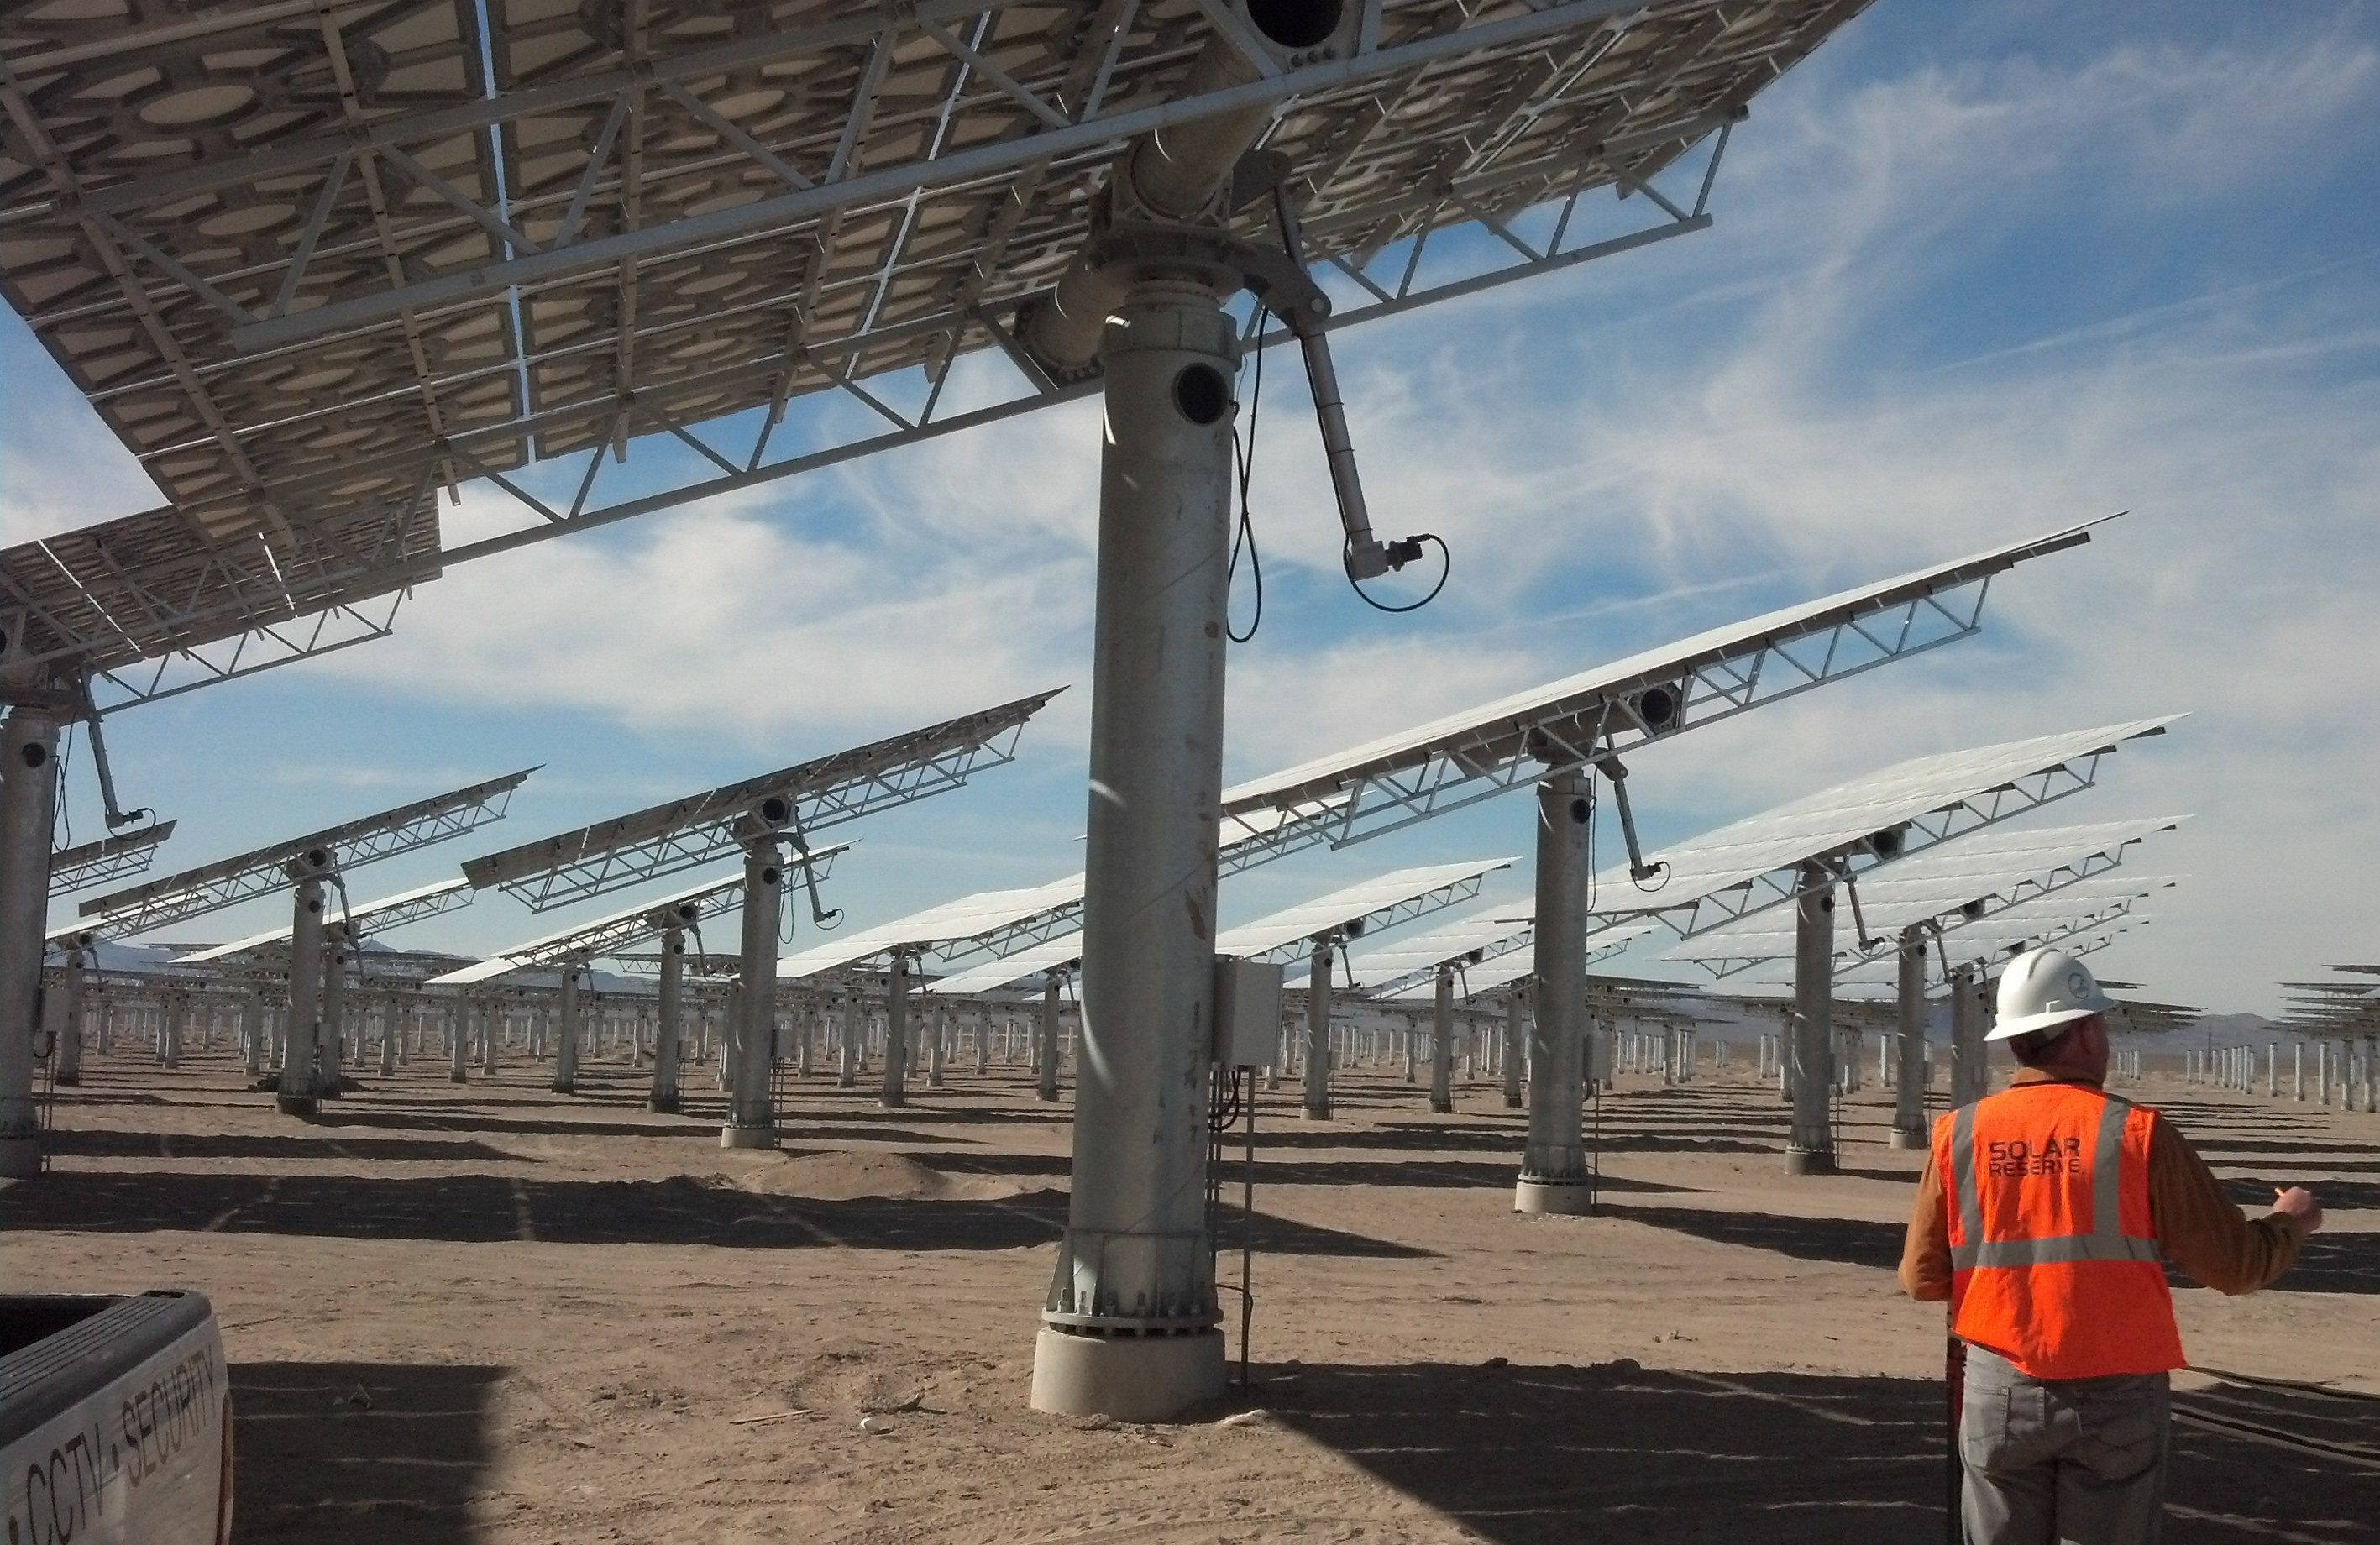
\includegraphics[width=.7\linewidth]{HeliostatImage.jpg}
\end{frame}

\begin{frame}
  \frametitle{As A Mechanical Engineer}
  \begin{itemize}
  \item Worked on the CDSEP plant performance model, integrating the Rocketdyne and Cobra Fortran code.
  \item Worked with the Photovoltaic team on power project development.
  \item Development of the PV performance model and design tool, and the systems engineering trades it allowed us to do quickly.
  \item Development of the CSP performance model/implementation of the smart dispatch logic in Matlab.
  \item Worked with the CSP team as well, mostly with Charles.
  \item Developed and troubleshot the financial model.
  \item Although this was a spreadsheet, I ended up learning a bit about project finance and internal return calculation.
  \end{itemize}
\end{frame}

% PV performance model development slide
\begin{frame}
  \frametitle{Photovoltaic Performance Toolkit Development}
  It would be pretty cool to make this kind of a ``web'' layout, rather than just bullets
  \begin{itemize}
  \item Inputs
  \item Outputs
  \item PVSyst or SAM based performance modeling
  \end{itemize}
\end{frame}

\begin{frame}
  \frametitle{PV System Design Tool}
  \begin{block}{Inputs}
    \begin{itemize}
      \item Land availability
      \item Module electrical characteristics
      \item Inverter electrical characteristics
      \item Interconnection voltage
    \end{itemize}
  \end{block}

  \begin{block}{Outputs}
    \begin{itemize}
    \item Estimated land usage
    \item Total array size
    \item Plant DC and AC capacities
      \item PVSyst or SAM input parameters
    \end{itemize}
  \end{block}
\end{frame}

\begin{frame}
  \frametitle{Performance Model}
  This was used to model interconnection losses, etc.

\end{frame}

%% All of the bullet points below deserve a slide
%TODO do a ``feature set'' drawing for the heliostat characterization to make it clearer how it works
\begin{frame}
  \frametitle{As A Systems Engineer}
  \begin{itemize}
  \item Development of the SR-120 control software (Matlab)
  \item Kalman filter development
  \item Include some stuff about the "zero" finding logic?
  \item Development of the SVS-Vistek and ViewWorks camera interfaces in C\#
  \item Test campaigns for the SR-120
  \item Determination and definition of performance requirements (IE mirror slope and pointing errors)
  \item Hands on testing at Sandia National Labs
  \item Troubleshooting and modifying the AMS software
  \item Camera and SPCA network setup 
  \item Daily SCRUMS (agile development) and piloting the system with Mark and Roger
  \item All of the performance data processing, which I had to automate because the rest of the team started on the SR-96
  \item Development of the in-situ/star characterization software
  \item Development of the control system interface; changing a relational object database into an object database
  \end{itemize}
\end{frame}

%% Slide on the SR-120 software development
\begin{frame}
  \frametitle{SR-120 Control Software Development}
  %% Zero finding and Kalman filter development
\end{frame}

\begin{frame}
  \frametitle{SR-120 Secondary Software Development}
  %% Camera and AMS software
\end{frame}

\begin{frame}
  \frametitle{Heliostat System Integration and Test}
  %% All of the testing campaigns at SNL
\end{frame}

\begin{frame}
  \frametitle{Crescent Dunes}
  %% This will cover star canting, with particular attention to the
  %% interface between the plant control system and the control software
\end{frame}

\subsection{Lockheed}
% I'm pretty sure the logo is copyrighted, so I shouldn't use it...
\begin{frame}
  \frametitle{Lockheed Martin Missiles and Fire Control}
  \center
  
\includegraphics[width=.7\linewidth]{LockheedLogo}
\end{frame}

\begin{frame}
  \frametitle{Affordability Test Bed}
  \begin{itemize}
  \item Describe what the ATB is and what it's intended to be
  \item Describe the loitering munition simulation and the image delay problem
  \item Software overlay generation/frame numbers
  \item Camera triggering
  \item Describe the oscilloscope testing to determine 
  \item Display port $\rightarrow$ DVI $\rightarrow$ HDMI $\rightarrow$ VGA $\rightarrow$ BNC 5 wire (RGB + HSYNC + VSYNC) $\rightarrow$ Alligator clips
  \item Show the frame delay histogram
  \end{itemize}
\end{frame}

\begin{frame}
  \frametitle{Loitering Munition Simulation}
  %% Describe the loitering munition simulation
  %% Continuous time simulation of a loitering munition
  %% Most of the sim and flight computer software is written in Simulink, and autocoded to c++
  %% All lower level stuff (frame handling, hardware interfaces) is written by hand in c++.  This is what I worked on.
\end{frame}

\begin{frame}
  \frametitle{Loitering Munition Frame Delay Problem}
  \begin{itemize}
  \item Discrepancies between simulation and reality
  \item Non-zero latency between an update of the simulation state (simulation time $t_{\tau}$) and when the image is rendered on the screen ($t_{\tau+\delta}$)
  \end{itemize}
\end{frame}

\begin{frame}
  \frametitle{PAC-3} % I might want to be a little sparing in my descriptions here, because this stuff is classified
  \begin{itemize}
  \item Intended to engage and destroy tactical ballistic missiles
  \item Most of it is classified
  \item Work on a Linux computing cluster on a continuous time simulation
  \item Integrating changes to the simulation from both internal, and also from the customer (IE the government), as well as the ground system components (which are from Raytheon).
  \item Integration of an older version of the simulation (entirely Fortran/Linux based) and modularizing it into several libraries which the customer can link together.  
  \item Builds on Windows or Linux
  \end{itemize}
\end{frame}


\begin{frame}
  \frametitle{Configuration Management on PACNET}

\end{frame}

%% A demo flow chart.
% Define block styles
\tikzstyle{decision} = [diamond, draw, fill=blue!20, 
    text width=4.5em, text badly centered, node distance=3cm, inner sep=0pt]
\tikzstyle{block} = [rectangle, draw, fill=blue!20, 
    text width=5em, text centered, rounded corners, minimum height=4em]
\tikzstyle{line} = [draw, -latex']
\tikzstyle{cloud} = [draw, ellipse,fill=red!20, node distance=3cm,
  minimum height=2em]

\begin{frame}
  \frametitle{Another flow chart}
  \center
  \resizebox{5.0cm}{!}{
\begin{tikzpicture}[node distance = 2cm, auto]
    % Place nodes
    \node [block] (init) {initialize model};
    \node [cloud, left of=init] (expert) {expert};
    \node [cloud, right of=init] (system) {system};
    \node [block, below of=init] (identify) {identify candidate models};
    \node [block, below of=identify] (evaluate) {evaluate candidate models};
    \node [block, left of=evaluate, node distance=3cm] (update) {update model};
    \node [decision, below of=evaluate] (decide) {is best candidate better?};
    \node [block, below of=decide, node distance=3cm] (stop) {stop};
    % Draw edges
    \path [line] (init) -- (identify);
    \path [line] (identify) -- (evaluate);
    \path [line] (evaluate) -- (decide);
    \path [line] (decide) -| node [near start] {yes} (update);
    \path [line] (update) |- (identify);
    \path [line] (decide) -- node {no}(stop);
    \path [line,dashed] (expert) -- (init);
    \path [line,dashed] (system) -- (init);
    \path [line,dashed] (system) |- (evaluate);
\end{tikzpicture}
}
\end{frame}

\begin{frame}
\Huge{\centerline{Q\&A?}}
\end{frame}

\end{document}
